% LaTeX template for ENGR1000J Summer 2025 Final Project Report
% Fully conforms to the provided Word template and formatting guidelines

\documentclass[10pt]{article}
\usepackage{CJKutf8}
\usepackage{times}
\usepackage{setspace}
\usepackage{graphicx}
\usepackage{caption}
\usepackage{tocloft}
\usepackage{titlesec}
\usepackage{parskip}
\usepackage{booktabs}
\usepackage{longtable}
\usepackage{hyperref}
\usepackage{xcolor}
\usepackage[letterpaper, margin=1in]{geometry}
\usepackage{fancyhdr}
\usepackage[export]{adjustbox} % 支持 valign 垂直对齐
\usepackage{parskip}
\usepackage[square, numbers]{natbib}
\usepackage{setspace} % 控制行距

% 定义“首页”页脚样式
\fancypagestyle{firstpage}{ \fancyhf{} % 清空默认内容
\fancyfoot{ \parbox{\textwidth}{\large\centering \textcolor{gray}{ ${}^{1}$ University of Michigan -- Shanghai Jiao Tong University Joint Institute\\ ${}^{2}$ Another Institute if applicable } } } \renewcommand{\footrulewidth}{0pt} \renewcommand{\headrulewidth}{0pt} }

% 定义“常规页”页脚样式
\fancypagestyle{mystyle}{ \fancyhf{} % 清空默认内容
\fancyfoot{ \noindent \begin{tabular*}{\textwidth}{@{\extracolsep{\fill}}cccc@{}}\adjustbox{valign=c}{
\includegraphics[height=0.3in]{figures/JI logo.png}} & \adjustbox{valign=c}{
\includegraphics[height=0.4in]{figures/team logo.png}} & \adjustbox{valign=c}{\small \textcolor{gray}{\begin{tabular}{@{}l@{}}Instructors: \\ Dr. Yanfeng Shen \\ Dr. Ting Sun\end{tabular}}} & \adjustbox{valign=c}{\raggedleft\small \textcolor{gray}{Page \textbf{\thepage} of 13}}\end{tabular*} } \renewcommand{\footrulewidth}{0pt} % 不显示常规页页脚分隔线
\renewcommand{\headrulewidth}{0pt} }

% 设置默认页脚样式为 "mystyle"

% Paragraph formatting
\setlength{\parindent}{0pt} % No indentation

% 设置段前、段后间距和固定行距
\setlength{\parskip}{10pt} % 段后10磅
\AtBeginDocument{ \linespread{1}%
\setlength{\baselineskip}{13pt}%
\let\latexoriginalpar\par
%\renewcommand{\par}{\vspace*{12pt}\latexoriginalpar}%
}

% Caption formatting
\captionsetup[figure]{labelfont=bf,labelsep=space,justification=justified,font=small,skip=6pt}
\captionsetup[table]{labelfont=bf,labelsep=space,justification=justified,font=small,skip=6pt}
% Ensure captions end with a period
%
% Section title formatting
\titleformat{\section}{\normalfont\Large\bfseries}{\thesection.}{1em}{}
\titleformat{\subsection}{\normalfont\large\bfseries}{\thesubsection.}{1em}{}

% Table of contents spacing
\setlength{\cftbeforesecskip}{4pt}
\setlength{\cftbeforetoctitleskip}{0pt}

% Reference font size
\renewcommand{\bibfont}{\small}

% No blank spaces at page bottoms
\raggedbottom

% Main content
\begin{document}
  \thispagestyle{firstpage}
  
\includegraphics[height=0.8in]{figures/headlogo.png}
  \\ \textbf{\Large ENGR1000J Introduction to Engineering, Summer 2025}\\[0.5em]
  \textbf{{\Large \today}}\\[1em]
  % Title block on first page
  \begin{center}
    % Logos side by side
    \begin{minipage}{0.45\textwidth}
      \centering
      
\includegraphics[height=1in]{figures/team logo.png}
    \end{minipage}\hfill
    \begin{minipage}{0.45\textwidth}
      \textbf{\Large Group 0: TC team}
    \end{minipage}\\[1em]
  \end{center}

  \noindent
  {\color{gray!30}\rule{\textwidth}{0.1pt}}

  {\Huge Project Title}
  % Graphical abstract placeholder

  {
\includegraphics[height=3in]{figures/preface_picture.png}}

  % Team members
  Team Member${}^{1}$ (\begin{CJK}
    {UTF8}{gbsn} 中文名
  \end{CJK}), ${}^{1}$, \textit{\underline {email@address}}

  Zeyi Chen${}^{1}$ (\begin{CJK}
    {UTF8}{gbsn} 陈泽奕
  \end{CJK}),
  $\textit{\underline{\href{mailto:marzich_44@sjtu.edu.cn}{marzich\_44@sjtu.edu.cn}}
  }$

  Xinchang Wang${}^{1}$ (\begin{CJK}
    {UTF8}{gbsn} 王欣畅
  \end{CJK}),
  $\textit{\underline{\href{mailto:wang_xinchang@sjtu.edu.cn}{wang\_xinchang@sjtu.edu.cn}}
  }$

  Different Institute Member ${}^{2}$, \textit{\underline {email@address}}
  % 在第一页内容后切换为常规页脚

  \newpage
  \pagestyle{mystyle}
  % Abstract
  \section*{Abstract}
  \addcontentsline{toc}{section}{Abstract}
  One paragraph (200--400 words) summarizing background, objectives, methods,
  key observations, conclusions, and significance.

  % Acknowledgments
  \section*{Acknowledgments}
  \addcontentsline{toc}{section}{Acknowledgments}
  Thank all parties who assisted this project, such as TAs, instructors, companies,
  and teammates.
  \newpage
  % Table of Contents
  \tableofcontents
  \thispagestyle{mystyle}
  \newpage

  % Main sections
  \section{Introduction}
  This section gives the reader a flavor of the work or project presented: the context
  of the work, the objectives, scope. In another word, the problem, the need, and
  the solution. Normally it begins with more general background, then gradually narrows
  down to a particular problem. After clearly identify the problem, what is needed
  will be liberated followed by a solution (brief summary of what your prototype
  can offer). The main goal of this section is to establish the significance of
  your project--why is it needed. (page limit 2 pages)

  Background is where you set the context for your work. You need to place your
  work in a context beyond the immediate engineering application. Current societal
  topics are a good place to start: security, energy, sustainability, productivity,
  etc. Spend some time discussing the broader engineering issues, then gradually
  narrow the discussion down to the technical side of your project. Background can
  include reasonable technical discussions on some fundamental theories related to
  your project. Please avoid your own personal opinion and keep all the
  discussions objective.

  Proper citation is always required per academic ethic and HC. List and number all
  references at the end of the report. Reference citations in the text should be
  in numerical order. [e.g., \citep{brandis2016nonequi}.].

  \textbf{Statements}
  \begin{itemize}
    \item Problem: clearly and concisely sums up what is the problem.

    \item Need/s: clearly and concisely sums up what is/are needed.

    \item Solution/s: clearly and concisely sums up the solution your project
      offers.
  \end{itemize}

  \section{Project Management}

  This section describes how your team managed this project. It should include a
  simple Gantt Chart, material budget, personnel information and contribution,
  and risk assessment. The tasks stated in the Gantt Chart correspond to the needs/solutions
  of this project.

  A Gantt chart provides concise but accurate information on the expected timetable
  for the project. The time for completion of each task should correspond
  exactly to the tasks previously described. Keep your Gantt Charts simple; as
  this graphic is intended for external audience, do not include too many tasks or
  descriptions of each task.

  Budget: State the proposed costs and budget of the project. Also include information
  on how you intend to manage the budget. One common way of showing the budget
  is according to the tasks as in Table \ref{tab:budget}.

  In building a set-up or prototype, material costs are typically accounted for in
  a bill of materials (BOM). This typically takes the form of the example shown
  below in Table \ref{tab:bill_of_materials}. State the costs of the project in an
  itemized form. Use a table, and make sure you list the total and any relevant sources
  for your purchases. If the purchasing link list is too long to fit in the main
  report body, you may include them as an appendix or a supplementary session.

  \begin{figure}[!ht]
    \centering
    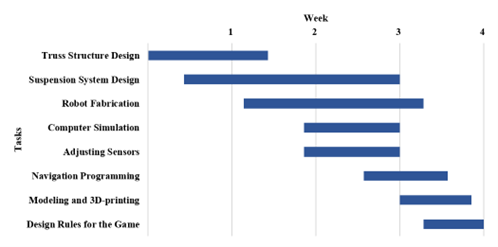
\includegraphics[width=0.8\textwidth]{figures/gantt_chart.png}
    \caption{Gantt chart for the project.}
    \label{fig:gantt_chart}
  \end{figure}

  \begin{table}[h]
    \centering
    \caption{Project estimated budget}
    \begin{tabular}{p{0.15\textwidth} p{0.45\textwidth} p{0.3\textwidth}}
      \toprule \textbf{Task} & \textbf{Description of work}        & \textbf{Anticipated costs, Yuan} \\
      \midrule 1             & 3D-printing container               & 150.00                           \\
      2                      & Construction of suspension system   & 100.00                           \\
      3                      & Realisation of automatic navigation & 200.00                           \\
      4                      & Construction of jogging system      & 200.00                           \\
      5                      & Realisation of additional function  & 200.00                           \\
      6                      & Tools                               & 150.00                           \\
      \midrule               & \textbf{Total}                      & \textbf{1000.00}                 \\
      \bottomrule
    \end{tabular}
    \label{tab:budget}
  \end{table}

  \begin{table}[!ht]
    \centering
    \caption{Bill of Materials.}
    \begin{tabular}{ccccr}
      \toprule Qty & Part Description & Vendor  & Part No. & Price (RMB) \\
      \midrule 8   & Wheel            & Vendor1 & --       & 5.70        \\
      \dots        & \dots            & \dots   & \dots    & \dots       \\
      \bottomrule
    \end{tabular}
    \label{tab:bill_of_materials}
  \end{table}

  Personnel: List the key personnel responsible for completion of the project,
  as well as other personnel involved in the project. Include brief summaries of
  their principal roles. These roles/contributions listed for each personnel
  shall be coherent with the tasks shown in Gantt Chart. The contributions of each
  team member are to be in agreement among the complete team, therefore, a signature
  is required from each member to endorse the content. (See Table 3).

  Risk Assessment: What needs to be in place for your project to succeed? What
  are the major sources of risk and how will you attempt to mitigate them? What is
  your fallback plan? What might be safety concerns?

  \section{System Design and Assembly}
  Provide schematic, component details, assembly steps.

  \section{Measurement Results and Discussion}
  Present results with figures and tables. Analyze and interpret critically.

  \section{Conclusions}
  Summarize achievements, objectives met, lessons learned, future work.

  \bibliographystyle{new-aiaa} % 使用你提供的样式文件
  \bibliography{sample} % 引用 references.bib 文件

  \newpage
  \appendix
  \section{Appendix}
  Additional materials and data.

  \newpage
  \section{Supplementary}
\end{document}